% Options for packages loaded elsewhere
\PassOptionsToPackage{unicode}{hyperref}
\PassOptionsToPackage{hyphens}{url}
%
\documentclass[
]{article}
\usepackage{amsmath,amssymb}
\usepackage{lmodern}
\usepackage{ifxetex,ifluatex}
\ifnum 0\ifxetex 1\fi\ifluatex 1\fi=0 % if pdftex
  \usepackage[T1]{fontenc}
  \usepackage[utf8]{inputenc}
  \usepackage{textcomp} % provide euro and other symbols
\else % if luatex or xetex
  \usepackage{unicode-math}
  \defaultfontfeatures{Scale=MatchLowercase}
  \defaultfontfeatures[\rmfamily]{Ligatures=TeX,Scale=1}
\fi
% Use upquote if available, for straight quotes in verbatim environments
\IfFileExists{upquote.sty}{\usepackage{upquote}}{}
\IfFileExists{microtype.sty}{% use microtype if available
  \usepackage[]{microtype}
  \UseMicrotypeSet[protrusion]{basicmath} % disable protrusion for tt fonts
}{}
\makeatletter
\@ifundefined{KOMAClassName}{% if non-KOMA class
  \IfFileExists{parskip.sty}{%
    \usepackage{parskip}
  }{% else
    \setlength{\parindent}{0pt}
    \setlength{\parskip}{6pt plus 2pt minus 1pt}}
}{% if KOMA class
  \KOMAoptions{parskip=half}}
\makeatother
\usepackage{xcolor}
\IfFileExists{xurl.sty}{\usepackage{xurl}}{} % add URL line breaks if available
\IfFileExists{bookmark.sty}{\usepackage{bookmark}}{\usepackage{hyperref}}
\hypersetup{
  pdftitle={Виды-индикаторы водных масс в Обской губе},
  hidelinks,
  pdfcreator={LaTeX via pandoc}}
\urlstyle{same} % disable monospaced font for URLs
\usepackage[margin=1in]{geometry}
\usepackage{longtable,booktabs,array}
\usepackage{calc} % for calculating minipage widths
% Correct order of tables after \paragraph or \subparagraph
\usepackage{etoolbox}
\makeatletter
\patchcmd\longtable{\par}{\if@noskipsec\mbox{}\fi\par}{}{}
\makeatother
% Allow footnotes in longtable head/foot
\IfFileExists{footnotehyper.sty}{\usepackage{footnotehyper}}{\usepackage{footnote}}
\makesavenoteenv{longtable}
\usepackage{graphicx}
\makeatletter
\def\maxwidth{\ifdim\Gin@nat@width>\linewidth\linewidth\else\Gin@nat@width\fi}
\def\maxheight{\ifdim\Gin@nat@height>\textheight\textheight\else\Gin@nat@height\fi}
\makeatother
% Scale images if necessary, so that they will not overflow the page
% margins by default, and it is still possible to overwrite the defaults
% using explicit options in \includegraphics[width, height, ...]{}
\setkeys{Gin}{width=\maxwidth,height=\maxheight,keepaspectratio}
% Set default figure placement to htbp
\makeatletter
\def\fps@figure{htbp}
\makeatother
\setlength{\emergencystretch}{3em} % prevent overfull lines
\providecommand{\tightlist}{%
  \setlength{\itemsep}{0pt}\setlength{\parskip}{0pt}}
\setcounter{secnumdepth}{-\maxdimen} % remove section numbering
\ifluatex
  \usepackage{selnolig}  % disable illegal ligatures
\fi

\title{Виды-индикаторы водных масс в Обской губе}
\author{}
\date{\vspace{-2.5em}}

\begin{document}
\maketitle

\hypertarget{ux432ux43eux434ux43dux44bux435-ux43cux430ux441ux441ux44b-ux432-ux43eux431ux441ux43aux43eux439-ux433ux443ux431ux435}{%
\subsection{Водные массы в Обской
губе}\label{ux432ux43eux434ux43dux44bux435-ux43cux430ux441ux441ux44b-ux432-ux43eux431ux441ux43aux43eux439-ux433ux443ux431ux435}}

Как и в любом эстуарии, водные массы в Обской губе имеют двойственное
происхождение: морское и речное. Имеющийся в распоряжении материал
позволяет лишь приблизительно охарактеризовать параметры водных масс.
При этом очевидное для эстуариев слоистое расположение водных масс
(вертикальный градиент) осложняется в акватории Обской губы, имеющей
довольно большую географическую протяженность, еще и горизонтальным
градиентом. Водная масса речного происхождения занимает всю толщу воды в
южной части акватории, а морская - в северной. Однако в средней части
слои водных масс могут сменять друг друга во времени, занимая разные
горизонты глубины. В связи с этим, объективный анализ водных масс, на
имеющемся материале, возможен только при анализе придонной части водного
тела. Распределение придонной солености в зависимости от глубины
(Рисунок 1), действительно, позволяет выделить несколько групп точек,
соответствующих трем водным массам, границы между которыми, на данном
этапе исследования, условны:

\begin{itemize}
\tightlist
\item
  Водная масса речного происхождения (соленость меньше 5 промилле);
\item
  Водная масса морского происхождения (соленость более 15 промилле);
\item
  Промежуточная водная масса (соленость от 5 до 15 промилле).
\end{itemize}

Придонная вода речного происхождения была отмечена на следующих
станциях: O101, O102, O104, O105, O107, O109, O111, O112, O13, O47, O50,
O51, O52, O55, O56, O58, O61, O62, O65, O67, O68, O71, O76, O77, O78,
O81, O83, O86, O87, O88, O89, O92, O95, O96, O97, O98, O99.

Придонная вода морского происхождения была отмечена на следующих
станциях: O1, O10, O11, O12, O14, O15, O16, O18, O19, O2, O21, O22, O24,
O25, O27, O28, O29, O3, O30, O32, O33, O34, O35, O36, O37, O38, O39, O4,
O40, O41, O42, O43, O44, O45, O46, O48, O49, O5, O53, O6, O60, O7, O8,
O9.

Придонная вода промежуточного типа была отмечена на следующих станциях:
O1, O10, O11, O12, O14, O15, O16, O18, O19, O2, O21, O22, O24, O25, O27,
O28, O29, O3, O30, O32, O33, O34, O35, O36, O37, O38, O39, O4, O40, O41,
O42, O43, O44, O45, O46, O48, O49, O5, O53, O6, O60, O7, O8, O9.

Следует отметить, что промежуточная водная масса привязана к наибольшим
глубинам. Возможно, что это опресненная вода морского происхождения,
сохранившаяся в ямах со времени захода в акваторию языка морской воды.

\begin{figure}
\centering
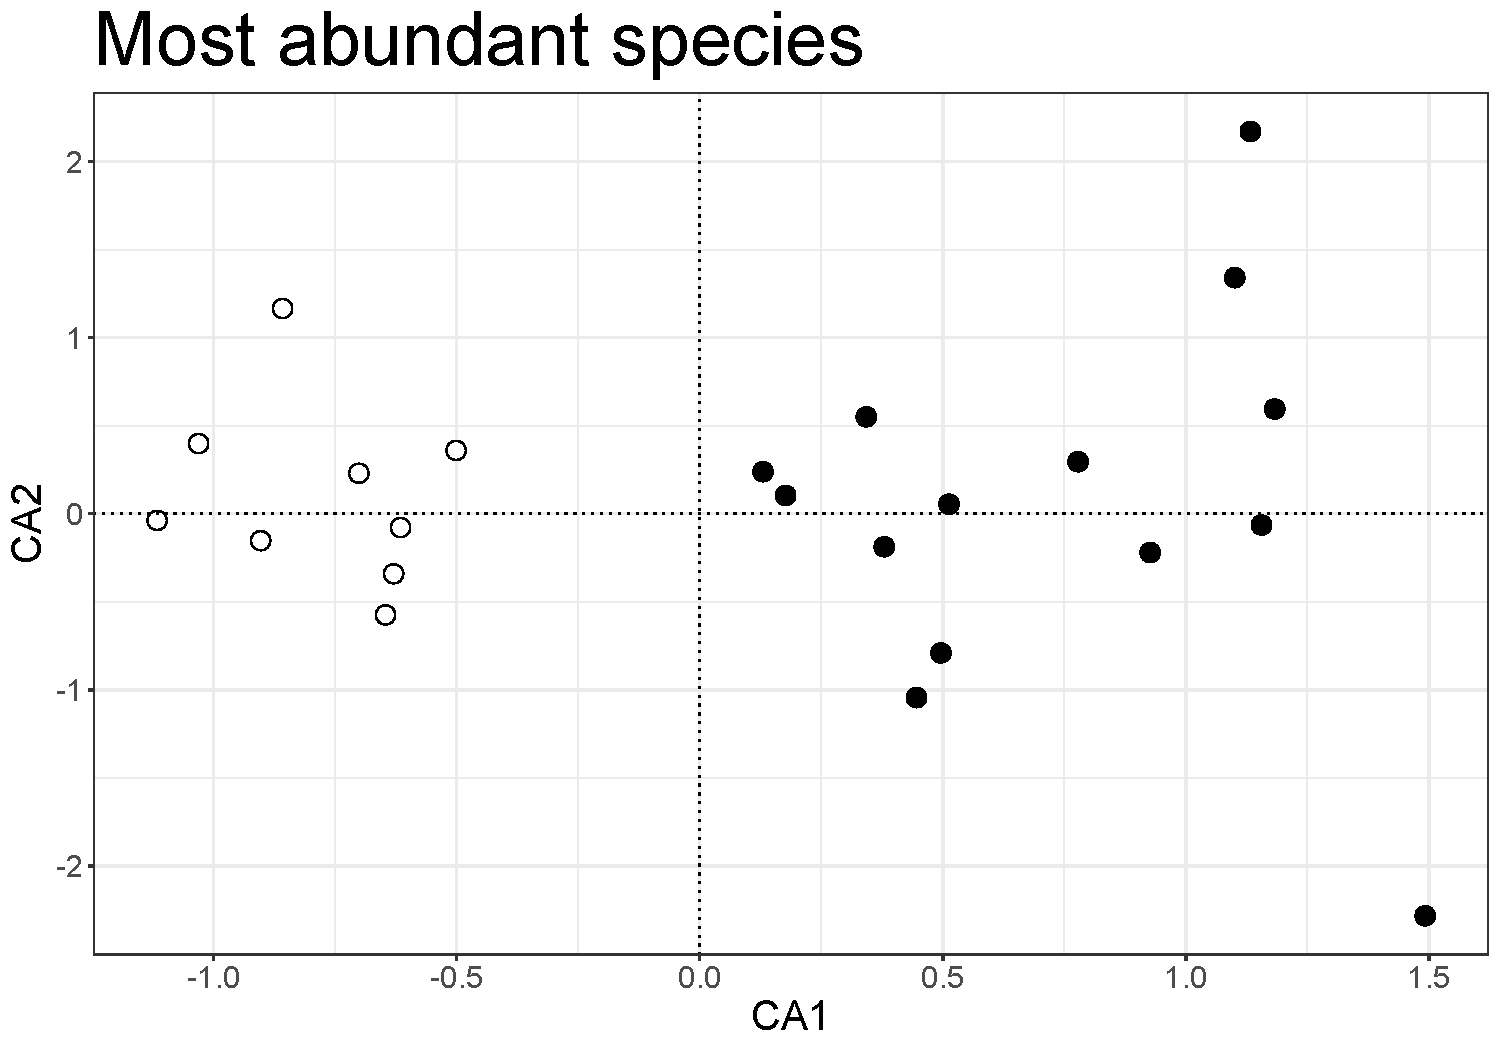
\includegraphics{Obskaya_bay_salinity_tolerant_files/figure-latex/unnamed-chunk-7-1.pdf}
\caption{\textbf{Рисунок 1.} Соленость придонного слоя воды на разных
глубинах Обской губы}
\end{figure}

\hypertarget{ux432ux438ux434ux44b-ux444ux438ux442ux43eux43fux43bux430ux43dux43aux442ux43eux43dux430-ux438ux43dux434ux438ux43aux430ux442ux43eux440ux44b-ux432ux43eux434ux43dux44bux445-ux43cux430ux441ux441}{%
\subsection{Виды фитопланктона индикаторы водных
масс}\label{ux432ux438ux434ux44b-ux444ux438ux442ux43eux43fux43bux430ux43dux43aux442ux43eux43dux430-ux438ux43dux434ux438ux43aux430ux442ux43eux440ux44b-ux432ux43eux434ux43dux44bux445-ux43cux430ux441ux441}}

Для выявления видов фитопланктона, характерных для морской и речной
водной массы была построена модель, описывающая распределение видов,
обнаруженных в придонном слое воды, в канонических корреспондентных
осях. В данной модели в качестве предиктора была использована только
соленость придонного слоя воды. Соответственно, первая, и единственная,
каноническая ось была связана с соленостью (Рисунок 2). Виды,
сосредоточенные в левой части ординации, - это организмы, обилие которых
достигает максимума при высокой солености. Противоположное положение на
ординации занимают виды, тяготеющие к водной массе речного
происхождения. Для выделения групп видов, наиболее сильно
скоррелированных с соленостью, в качестве границ, отсекающих их от
других видов, были взяты значения первого и третьего квартилей нагрузок
видов по первой канонической оси.

\begin{figure}
\centering
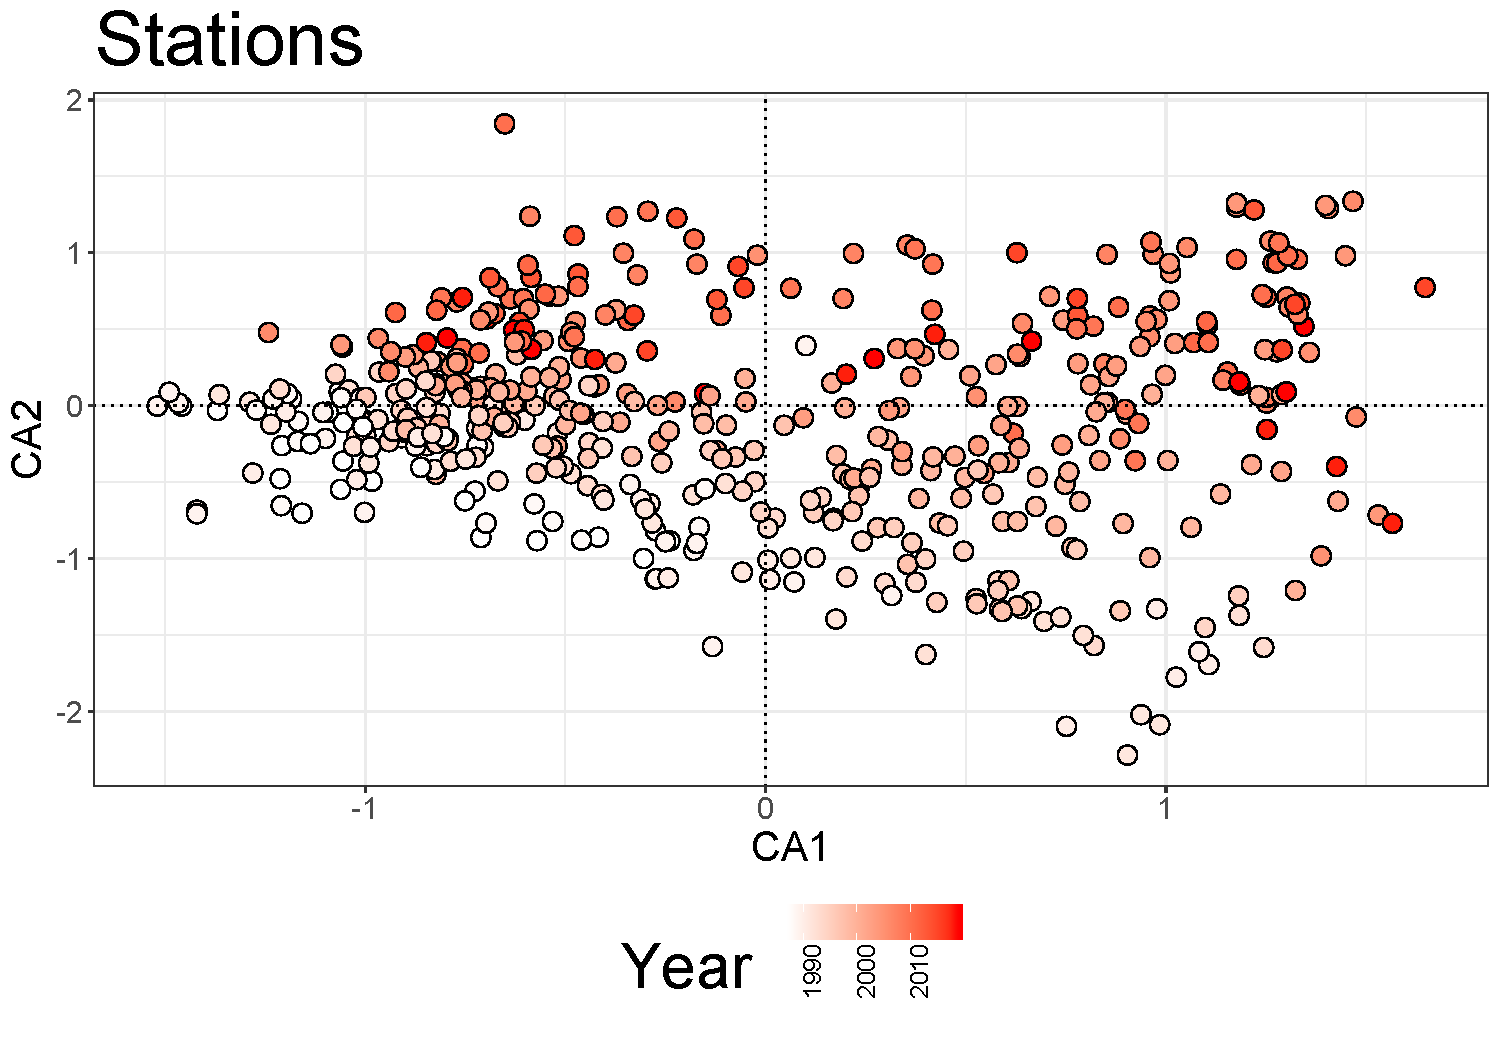
\includegraphics{Obskaya_bay_salinity_tolerant_files/figure-latex/unnamed-chunk-9-1.pdf}
\caption{\textbf{Рисунок 2.} Ординация видов фитопланктона вдоль первой
канонической оси и первой корреспондентной оси}
\end{figure}

Согласно введенному критерию разделения, к числу идикаторов морской
водной массы относятся следующие таксоны.

\begin{longtable}[]{@{}ll@{}}
\toprule
Виды & Таксон более высокого ранга \\
\midrule
\endhead
Amphidinium carterae & Dinophyta \\
Amphidinium sphenoides & Dinophyta \\
Anabaena spiroides & Cyanophyta \\
Caloneis sp. & Bacillariophyta \\
Chaetoceros danicus & Bacillariophyta \\
Chaetoceros socialis & Bacillariophyta \\
Chlamydomonas sp. & Chlorophyta \\
Closterium aciculare & Chlorophyta \\
Cyclotella choctawhatcheeana & Bacillariophyta \\
Dictyosphaerium sp. & Chlorophyta \\
Ebria tripartita & Chrysophyta \\
Eutreptiella lanowii & Euglenophyta \\
Gyrodinium lacryma & Dinophyta \\
Heterocapsa triquetra & Dinophyta \\
Karlodinium veneficum & Dinophyta \\
Katodinium glaucum & Dinophyta \\
Melosira dubia & Bacillariophyta \\
Monoraphidium mirrabile & Chlorophyta \\
Nizchia spp. & Bacillariophyta \\
Oocystis borgei & Chlorophyta \\
Oxytoxum gladiolus & Dinophyta \\
Oxytoxum scolopax & Dinophyta \\
Pediastrum biradiatum & Chlorophyta \\
Pediastrum boryanum v. longicornis & Chlorophyta \\
Peridiniella catenata & Dinophyta \\
Prorocentrum cordatum & Dinophyta \\
Prorocentrum micans & Dinophyta \\
Prorocentrum minimum & Dinophyta \\
Protoperidinium brevipes & Cryptophyta \\
Protoperidinium pellucidum & Cryptophyta \\
Pterosperma vanhoeffenii & Chlorophyta \\
Scenedesmus magnus & Chlorophyta \\
Scrippsiella trochoidea & Dinophyta \\
Stephanodiscus hantschii & Bacillariophyta \\
Teleaulax amphioxeia & Cryptophyta \\
Thalassionema nitzschioides & Bacillariophyta \\
Thalassiosira gravida & Bacillariophyta \\
\bottomrule
\end{longtable}

К числу индикаторов пресной водной массы относятся следующие формы.

\begin{longtable}[]{@{}ll@{}}
\toprule
Виды & Таксон более высокого ранга \\
\midrule
\endhead
Actinocyclus normanii & Bacillariophyta \\
Amphora ovalis & Bacillariophyta \\
Aphanizomenon sp. & Cyanophyta \\
Aulacoseira islandica & Bacillariophyta \\
Aulacoseira italica & Bacillariophyta \\
Craticula halophila & Bacillariophyta \\
Crucigenia quadrata & Chlorophyta \\
Cryptomonas gracilis & Cryptophyta \\
Cryptomonas ovata & Cryptophyta \\
Cyclotella sp. & Bacillariophyta \\
Cylindrotheca closterium & Bacillariophyta \\
Cymatopleura solea & Bacillariophyta \\
Fragilaria construens & Bacillariophyta \\
Fragilaria crotonensis & Bacillariophyta \\
Fragilaria virescens & Bacillariophyta \\
Gymnodinium arcticum & Dinophyta \\
Heterocapsa rotundata & Dinophyta \\
Navicula directa & Bacillariophyta \\
Navicula septentrionalis & Bacillariophyta \\
Nitzschia communis & Bacillariophyta \\
Nitzschia linearis & Bacillariophyta \\
Nitzschia palea & Bacillariophyta \\
Nitzschia seriata & Bacillariophyta \\
Nitzschia spp. & Bacillariophyta \\
Nitzschia vermicularis & Bacillariophyta \\
Oscillatoria sp. & Cyanophyta \\
Planktothrix agardhii & Cyanophyta \\
Protoperidinium granii & Cryptophyta \\
Protoperidinium sp. & Cryptophyta \\
Scenedesmus spinosus & Chlorophyta \\
Stephanodiscus hantzschii & Bacillariophyta \\
Surirella elegans & Bacillariophyta \\
Surirella ovalis & Bacillariophyta \\
Surirella ovata & Bacillariophyta \\
Trachelomonas acanthostoma & Euglenophyta \\
Trachelomonas regulosa & Euglenophyta \\
Trachelomonas volvocina & Euglenophyta \\
\bottomrule
\end{longtable}

Суммарное обилие видов из обеих групп закономерно связано с типом водных
масс ( Рисунок 3). Важно отметить, что промежуточная водная масса, судя
по обилию индикаторов, скорее должна классифицироваться как
пресноводная.

\begin{figure}
\centering
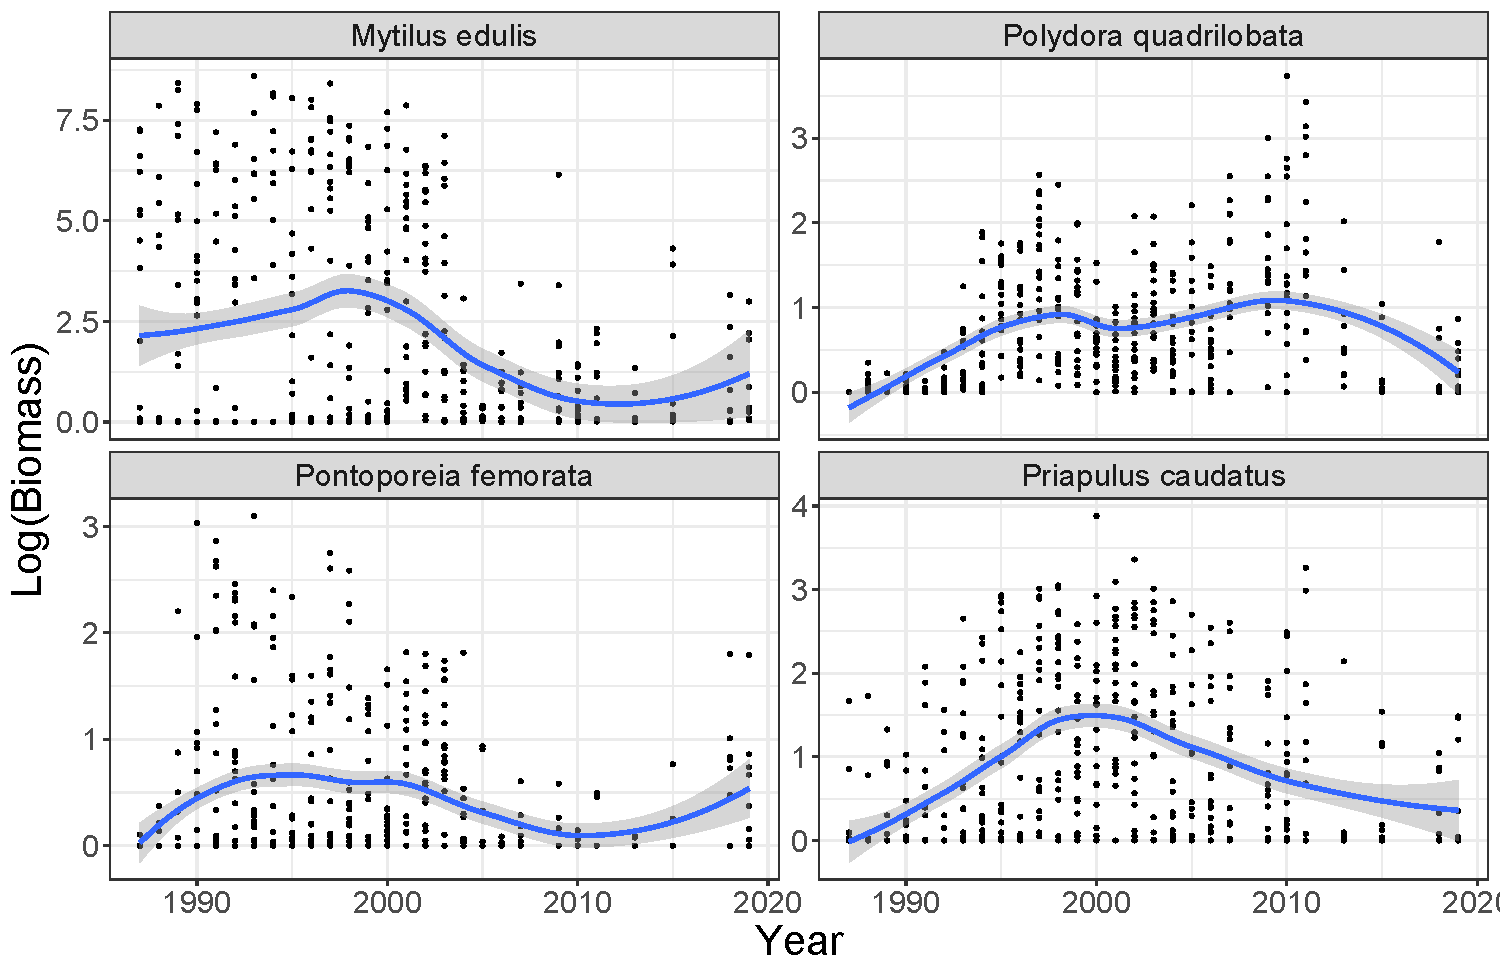
\includegraphics{Obskaya_bay_salinity_tolerant_files/figure-latex/unnamed-chunk-13-1.pdf}
\caption{\textbf{Рисунок 3.} Обилие видов-индикаторов из группы витов
фитопланктона в разных водных массах}
\end{figure}

\hypertarget{ux432ux438ux434ux44b-ux437ux43eux43eux43fux43bux430ux43dux43aux442ux43eux43dux430-ux438ux43dux434ux438ux43aux430ux442ux43eux440ux44b-ux432ux43eux434ux43dux44bux445-ux43cux430ux441ux441}{%
\subsection{Виды зоопланктона индикаторы водных
масс}\label{ux432ux438ux434ux44b-ux437ux43eux43eux43fux43bux430ux43dux43aux442ux43eux43dux430-ux438ux43dux434ux438ux43aux430ux442ux43eux440ux44b-ux432ux43eux434ux43dux44bux445-ux43cux430ux441ux441}}

Принцип выделения видов-индикаторов водных масс среди зоопланктона был
аналогичен описаному выше. Однако, поскольку сбор планктона проводился
во всей толще воды, то точной привязки к водным массам тех или иных
видов может не наблюдаться. Это связано с тем, что, при наличии
вертикальной стратификации водных масс, взятие пробы путем протяжки
через весь столб воды, приводит к смешению сообществ. Однако на
ординации достаточно четко выделяется две группы видов по-разному
связанными с соленостью (Рисунок 4)

\begin{figure}
\centering
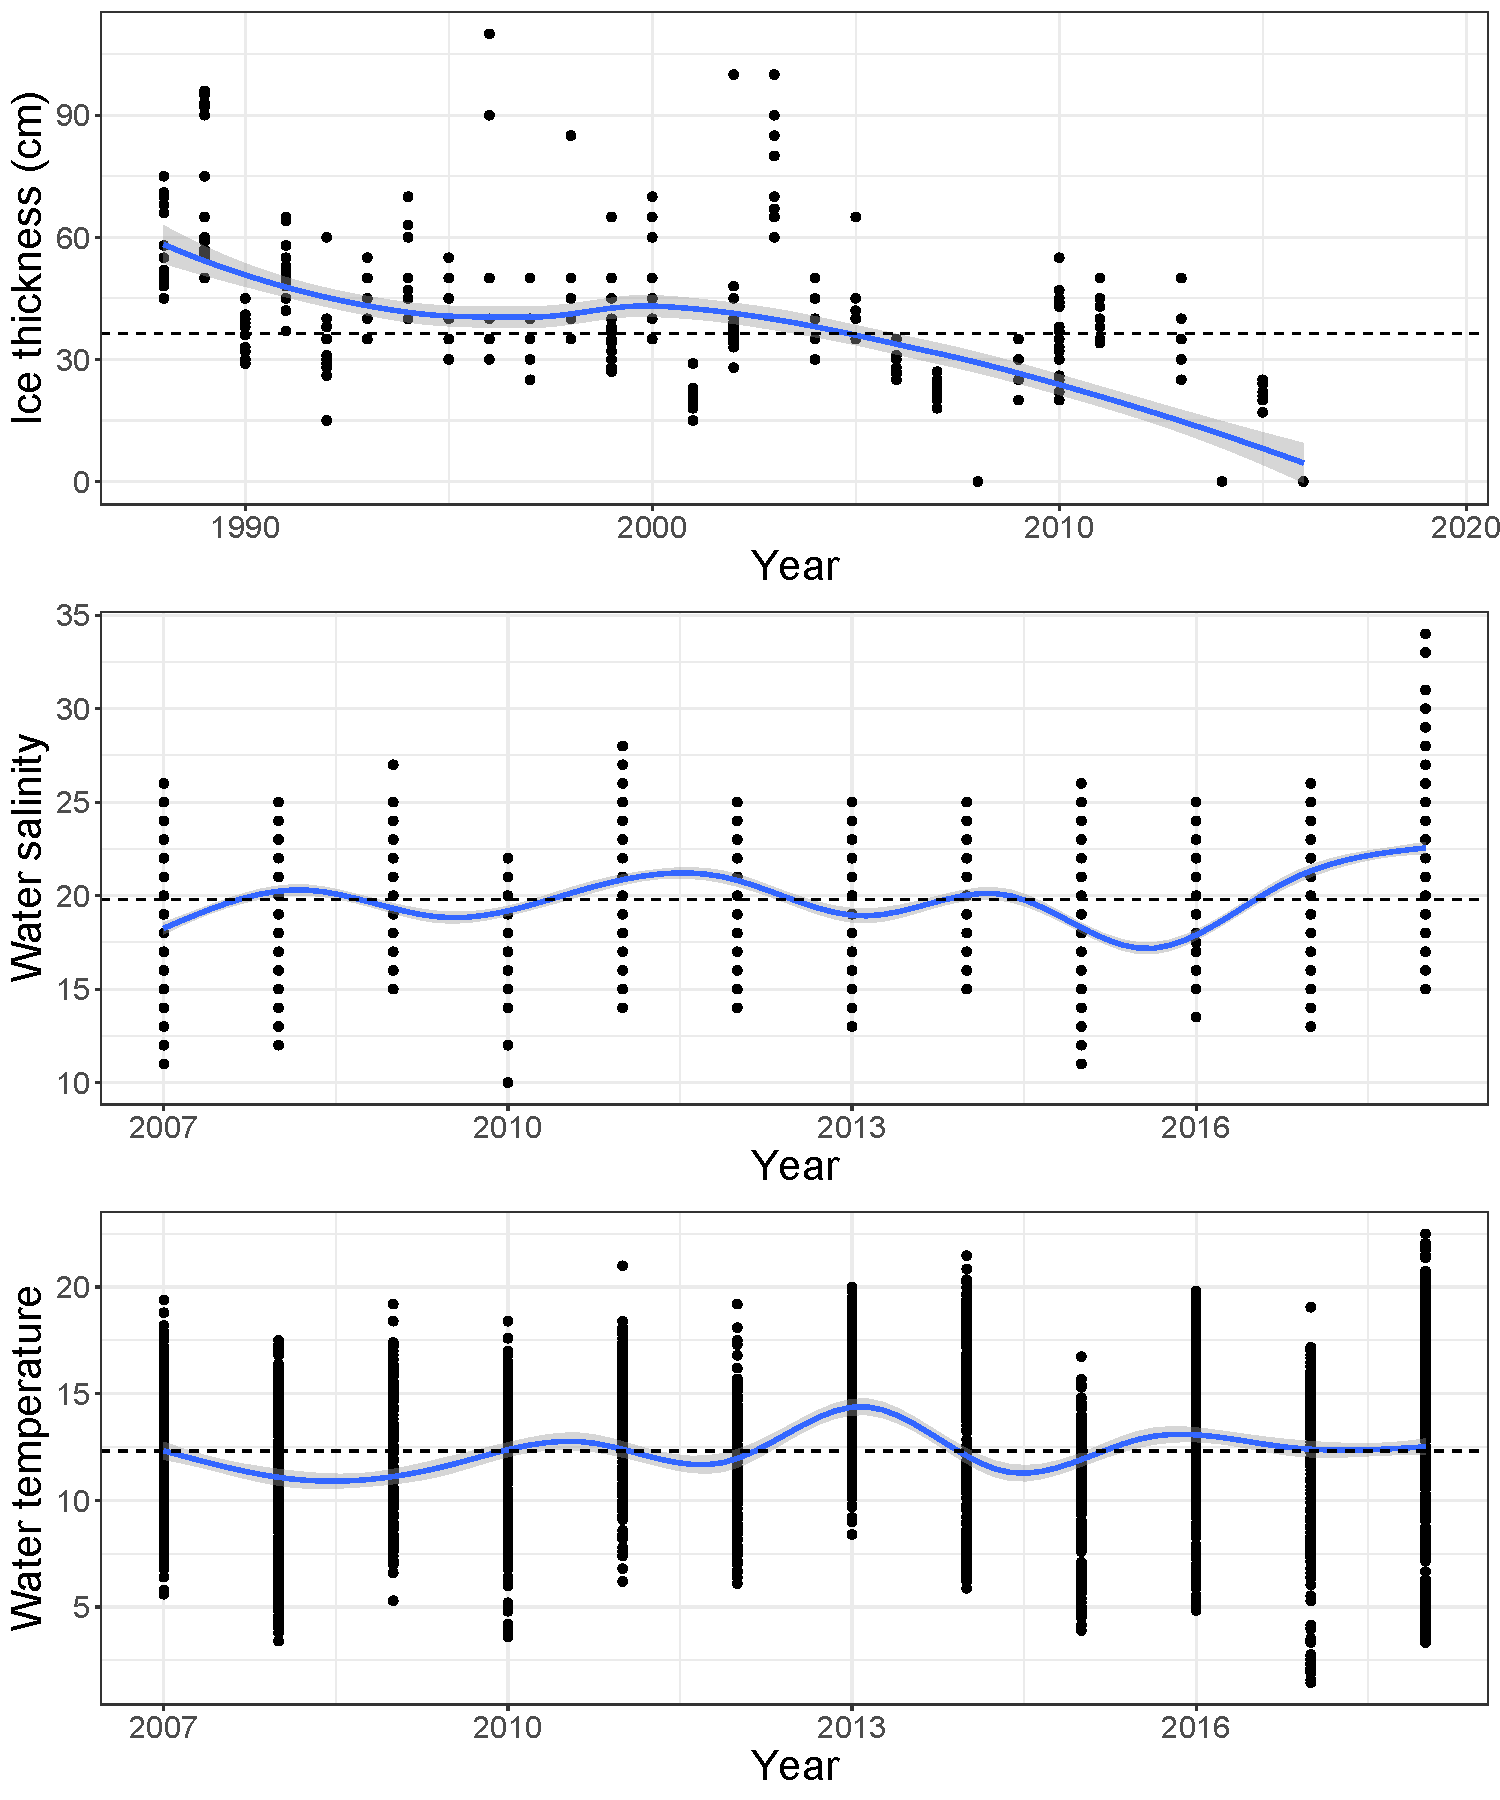
\includegraphics{Obskaya_bay_salinity_tolerant_files/figure-latex/unnamed-chunk-16-1.pdf}
\caption{\textbf{Рисунок 4.} Ординация видов зоопланктона вдоль первой
канонической оси и первой корреспондентной оси}
\end{figure}

Согласно введенному критерию разделения, к числу индикаторов морской
водной массы относятся следующие таксоны.

\begin{longtable}[]{@{}l@{}}
\toprule
Виды \\
\midrule
\endhead
Acartia longiremis \\
Aglantha digitale \\
Bivalvia larvae \\
Calanus finmarchicus \\
Calanus glacialis \\
Cerianthus sp. \\
Euphysa flammea \\
Harpacticus uniremis \\
Larvae Polychaeta \\
Mesochra lilljeborgii \\
Microsetella norvegica \\
Nauplia Temora \\
Obelia longissima \\
Oithona atlantica \\
Oithona similis \\
Podon leuckartii \\
Pseudocalanus acuspes \\
Pseudocalanus minutus \\
Senecella calanoides \\
Temora longicornis \\
\bottomrule
\end{longtable}

К числу индикаторов пресной водной массы относятся следующие формы.

\begin{longtable}[]{@{}l@{}}
\toprule
Виды \\
\midrule
\endhead
Acanthocyclops vernalis \\
Arctodiaptomus bacillifer \\
Bosmina longirostris \\
Brachionus angularis \\
Bythotrephes longimanus \\
Cyclops abyssorum \\
Cyclops scutifer \\
Diacyclops bisetotus \\
Eucyclops serrulatus \\
Eudiaptomus gracilis \\
Eurytemora lacustris \\
Keratella quadrata \\
Leptodora kindtii \\
Megacyclops viridis \\
Mesocyclops leuckarti \\
Microcyclops varicans \\
Notholca acuminata \\
Polyarthra dolichoptera \\
Synchaeta kitina \\
Trichocerca capucina \\
\bottomrule
\end{longtable}

Суммарное обилие видов из обеих групп закономерно связано с типом водных
масс ( Рисунок 5): виды-индикаторы водных масс речного происхождения
обильны лишь на станциях, где представлена пресная и промежуточная
водная масса, морские виды-индикаторы, соответственно, в водной массе
морского происхождения.

\begin{figure}
\centering
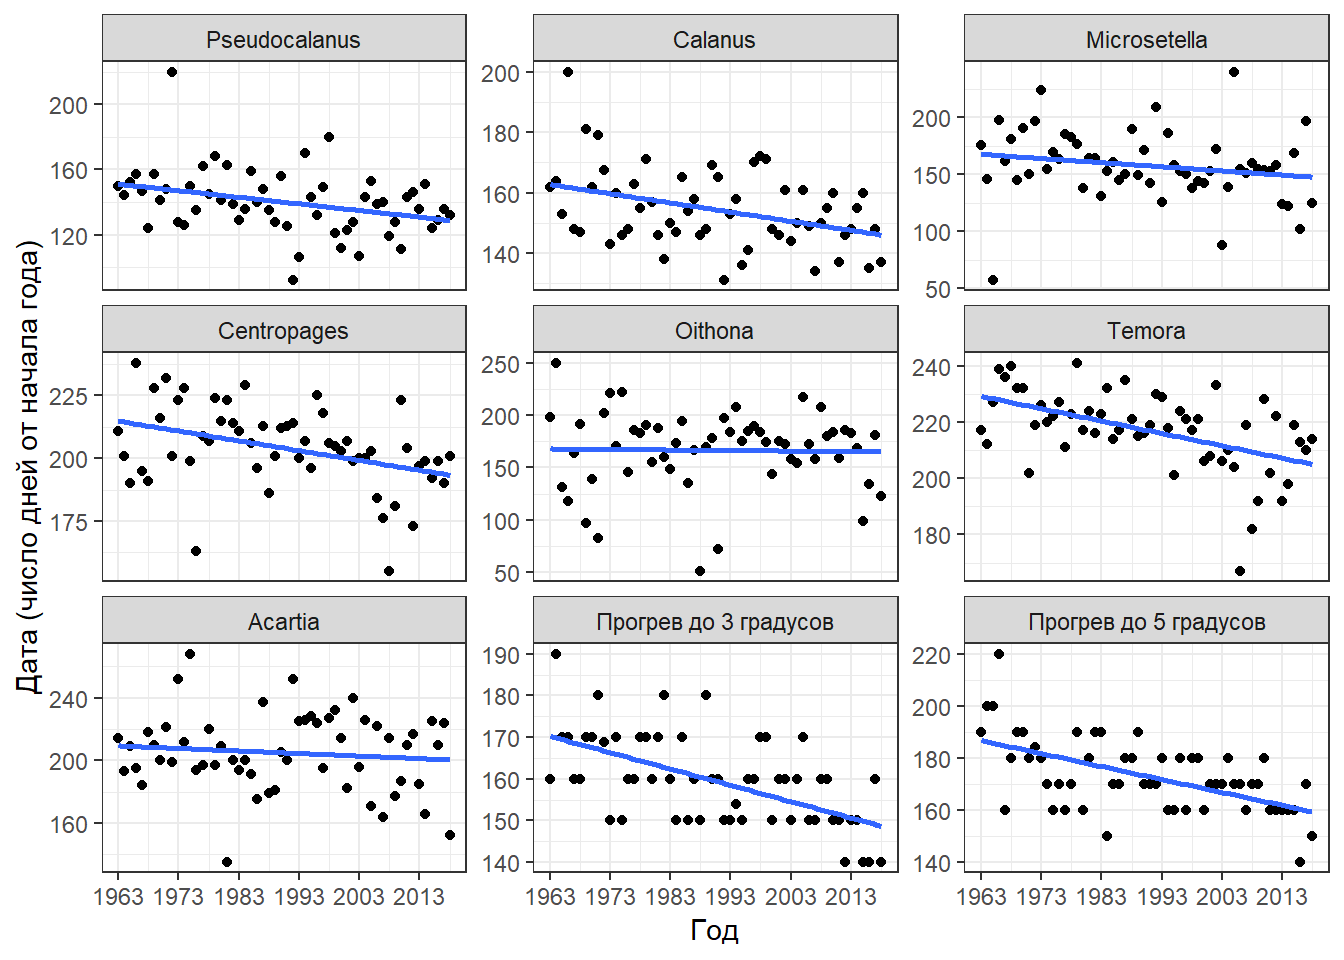
\includegraphics{Obskaya_bay_salinity_tolerant_files/figure-latex/unnamed-chunk-20-1.pdf}
\caption{\textbf{Рисунок 5.} Обилие видов-индикаторов из числа
зоопланктона в разных водных массах}
\end{figure}

\hypertarget{ux432ux438ux434ux44b-ux437ux43eux431ux435ux43dux442ux43eux441ux430-ux438ux43dux434ux438ux43aux430ux442ux43eux440ux44b-ux432ux43eux434ux43dux44bux445-ux43cux430ux441ux441}{%
\subsection{Виды зобентоса индикаторы водных
масс}\label{ux432ux438ux434ux44b-ux437ux43eux431ux435ux43dux442ux43eux441ux430-ux438ux43dux434ux438ux43aux430ux442ux43eux440ux44b-ux432ux43eux434ux43dux44bux445-ux43cux430ux441ux441}}

Поиск видов-индикаторов водных масс среди зообентоса должен
сопровождаться целым рядом оговорок. Во-первых, бентосные животные живут
дольше большинства планктонных организмов и, соответственно, их
популяции менее подвержены кратковременным изменениям, связанным с
перемещениями водных масс. Во-вторых, многие донные животные, обитающих
в эстуариях, являются осморегуляторами и обладают адаптациями,
позволяющими переносить значительные перепады солености. В-третьих,
соленость может быть заметным лимитирующим фактором только для морских
форм, пресноводные же многоклеточные организмы легче переносят
осолонение. Иными словами, увеличение притока пресной воды может быть
фатальным для морских форм, но заход морских вод в пресноводные участки
для бентосных организмов не столь чувствителен. В-четвертых, в
биоценотическом покрове дна в Обской губе очень выражено пятнистое
распределение организмов, связанное с локальными нарушениями разной
природы. Эта мозаика может маскировать градиенты, связанные с
распределением водных масс.

Все сказанное значительно сокращает вероятность правильного определения
роли видов, как индикаторов водных масс. Однако ординация, проведенная
по тем же принципам, что и в предыдущих случаях, позволяет увидеть четко
очерченную группу морских видов и несколько групп, связанных с
опресненными водами.

\begin{figure}
\centering
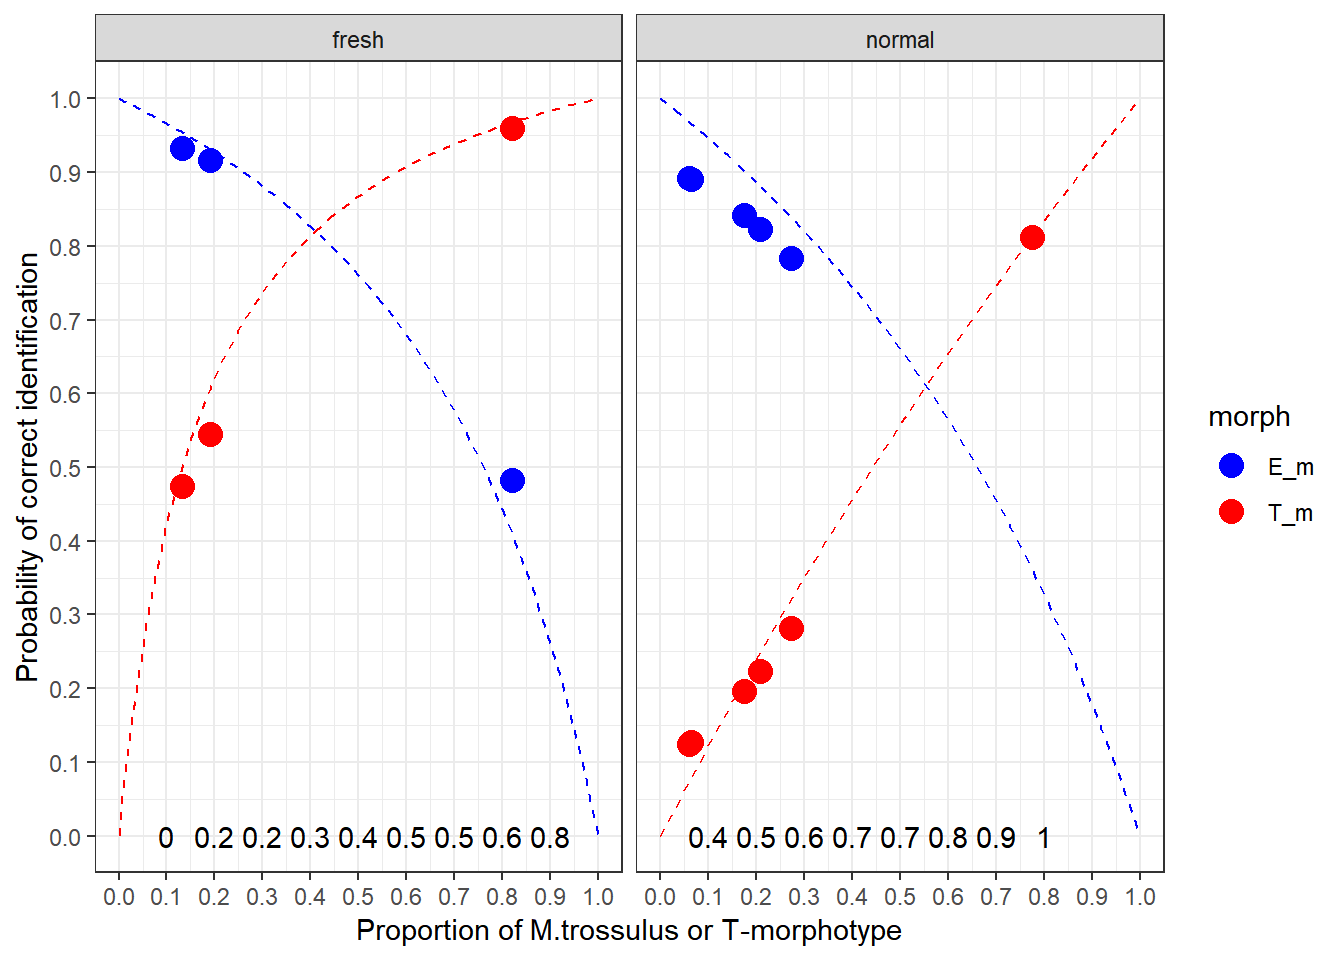
\includegraphics{Obskaya_bay_salinity_tolerant_files/figure-latex/unnamed-chunk-23-1.pdf}
\caption{\textbf{Рисунок 2.} Ординация видов зообентоса вдоль первой
канонической оси и первой корреспондентной оси. В анализе использованы
только обильные виды, включенные ранее в анализ сообществ зообентоса
(см. соответствующую часть отчета)}
\end{figure}

К числу индикаторов морской водной массы относятся следующие таксоны.

\begin{longtable}[]{@{}l@{}}
\toprule
Виды \\
\midrule
\endhead
Ampharete vega \\
Ostracoda gen. sp. \\
Diastylis sulcata \\
Pontoporeia femorata \\
\bottomrule
\end{longtable}

Опресненную водную массу маркируют следующие виды.

\begin{longtable}[]{@{}l@{}}
\toprule
Виды \\
\midrule
\endhead
Senecella siberica \\
Mysis relicta \\
Saduria entomon \\
Monoporeia affinis \\
\bottomrule
\end{longtable}

Подчеркнем еще раз, что эти формы, скорее, маркеры эстуарных условий,
чем пресноводных.

Суммарное обилие видов из обеих групп на станциях с придонной водой,
относящейся к разным водным массам ( Рисунок 6), как и в предыдущих
случаях, демонстрирует корреляцию с водными массами, однако эта связь
выражена заметно слабее, чем в случае с планктонными формами.

\begin{figure}
\centering
\includegraphics{Obskaya_bay_salinity_tolerant_files/figure-latex/unnamed-chunk-27-1.pdf}
\caption{\textbf{Рисунок 6.} Обилие видов-индикаторов зообентоса в
разных водных массах}
\end{figure}

\end{document}
